\chapter {Introduction} \label{ch:intro}

Until relatively recently, the extent and efficiency of planet formation around stars other than the Sun was a mystery. Gas and dust are known to collapse under the influence of gravity to form molecular clouds and eventually stellar cores, but the details surrounding the eventual fate of the extra material that does not make its way onto a star are much less clear. Clearly, the solar system was able to condense this material into a series of planets which have persisted for $\sim$ 4.5 billion years, but the question of whether this outcome is uniquely special and unusual, went unanswered until the Kepler Space Telescope was launched.

The latest population demographics \textbf{(for a review, see \cite{winn15})} from these planet-hunting missions make one thing clear: planet formation is ubiquitous. Not only do the majority of stars in our galaxy host planets, but many of these appear to be rocky, roughly Earth-sized and potentially habitable. \textbf{Recent work using planet population synthesis models shows that these exoplanetary systems can be categorized into four distinct classes \cite{emsenhuber23, mishra23a, mishra23b}}. One surprising result, however, is that many of these planetary systems bear little resemblance to the orbital arrangement of the solar system \textbf{\cite{raymond20}}. Instead, some of these systems are packed much more closely to their host stars and would lie entirely inside the orbit of Mercury if superimposed over the sun. Due to observational biases, this result is not entirely surprising (planets closer to their stars produce a stronger signal for transit and radial velocity measurements), but it highlights an important question: what happened to the solar system that didn't happen to these compact multiplanet systems? The answer to this question likely contains some important clues that can be used to build a more cohesive, global picture of the planet formation process.

\section{Pathways to Terrestrial Planet Formation}

The growth and eventual formation of terrestrial planets, which are classified by their composition of primarily rock and metal, is a process that spans a huge range of sizes in a bottom-up fashion \cite{safronov72}. This process beings with $\mu$m sized dust grains and eventually leads to gravitationally-bound bodies which are 1000's of km in size. Given the wide range of size scales that objects evolve through as they grow to form planets, there is a diverse collection of physical processes that must be considered and modeled to properly capture the possible outcomes of the terrestrial planet formation process.

At the smallest sizes, aerodynamic forces between solids and the gaseous component of the protoplanetary disk dominate growth. Material physics is important here, as grains sediment toward the disk midplane and occasionally collide with each other and stick \cite{okuzumi12, windmark12, garaud13, katoka13} to progressively form larger bodies.  Around mm size scales, however, a number of growth barriers are thought to present themselves. These include catastrophically short radial drift timescales \cite{adachi76, weidenschilling77}, problems with particles sticking to form larger objects and even destructive collisions \cite{windmark12}. \textbf{Because observational constraints on solids of these sizes in planet-forming disks are tenuous and often indirect, microgravity experiments involving dust grains and pebbles are providing a promising window into this phase of growth (see \cite{wurm21}).}

Despite these barriers to growth, terrestrial planet formation appears common \cite{bonfils13, dressing15, gaidos16}. This implies that some physical process must quickly and efficiently grow solids up to kilometer sizes, where gravity begins to dominate the physical interactions. These small gravitationally bound objects are referred to as \textit{planetesimals} and are usually taken to be the basic building blocks of terrestrial planets. In planet formation models, planetesimals are allowed to collide and grow, while gravitational interactions and aerodynamic drag from the residual gaseous disk alter their velocities. Although most planetesimals are eventually incorporated into planets, a small \textbf{number} can remain long after the system forms. In the solar system, these bodies eventually went on to populate the asteroid belt and Kuiper belt \cite{duncan89, bottke05, levison08, morbidelli09}. In some adolescent exoplanetary systems \textbf{(ranging from a few \cite{espaillat17} to hundreds \cite{mamajek12} of Myr in age}, dust from these colliding residual planetesimals is often observable \cite{wyatt08, gaspar20}.

A significant uncertainty in the final planet formation process involves determining whether and how far these building blocks move throughout the disk as they incorporate themselves into the final bodies. Although radial drift due to aerodynamic gas drag can be treated as a second-order effect for planetesimal and larger-sized objects, objects that reach roughly Mars-sized can stir up spiral density waves in the gas disk and lose significant amounts of angular momentum as they migrate inward \cite{ward97}. This has significant implications for the final orbital architecture of the planetary system, as the solid mass becomes much more centrally concentrated and planetary compositions consist of material that should be expected to condense much further from the central star. One key prediction of a migration-driven model is that planets should be expected to stop migrating and lock into mean-motion resonances once they reach the inner edge of the gaseous disk \cite{hands14}. A \textbf{small but} appreciable fraction of close-in terrestrial multiplanet systems are found in resonant chains \cite{gillon16, gillon17, christiansen18, agol21, leleu21}. However, resonant chain systems formed in this fashion are often not dynamically stable and this telltale signature of convergent migration is often only temporary \cite{terquem07, pierens11, izidoro17, mcnally19}.

Alternatively, large-scale migration due to tidal torques with the gas disk may play an insignificant role in shaping the final planetary configuration and terrestrial planets are formed largely \textit{in-situ}. In this scenario, the final properties of the planets themselves more closely reflect the conditions of the initial disk of solids (at least at the time of planetesimal formation). A common method to assess the viability of in-situ formation is to take an observed collection of planets, smear out the masses, and then evaluate the physicality of the inferred distribution of solids. This approach was first applied to the solar system to infer the natal distribution of solids (called the MMSN, or minimum-mass solar nebula) \cite{hayashi81} and has more recently been applied to compact multiplanet systems observed by Kepler \cite{chiang13, dai20}. One attractive feature of an in-situ model is it's relative simplicity to implement in planet formation models. Gravity and collisions are the two physical processes that dominate, both of which can easily be handled by modern N-body codes. Gas disk migration models, on the other hand, are still wrought with uncertainties that bring into question the strength, timing and even direction of migration that depend on both the exact mass distribution and thermodynamic properties of the gas disk \cite{ayliffe10, bitsch13, ogihara18}.

The wealth of information that recent missions like Kepler and TESS have provided about terrestrial planets is making one fact abundantly clear: a one-size-fits-all model for terrestrial planet formation is overly simplistic. In some cases, it it clear that in-situ formation cannot have operated \cite{raymond14}, while only a small fraction of systems have clearly undergone large-scale migration \cite{he22}. Given the limitations and uncertainties associated with current migration models, and the relative simplicity of growing gravitationally bound solids in-situ, a closer look at planetesimal accretion and eventual terrestrial planet formation using high resolution N-body simulations is warranted. Until recently, these types of simulations have required overly restrictive simplifications, such as starting with fully-formed Mars-sized planetary embryos, or ignoring gravitational interactions between smaller bodies. In this thesis, I present some of the first simulations that are free of these limitations and use the results to understand small body populations in the present day solar system, collisionally generated dust around young planetary systems and compact multi planet systems observed by Kepler and TESS (also known as STIPs, or systems of tightly-packed inner planets).

\section{Planetesimal Formation}

As mentioned above, the barriers to growth for mm-sized bodies due to radial drift, bouncing and fragmentation suggest that continued growth through cm and meter sizes must proceed in a qualitatively different fashion. For mm-sized objects, equal mass collisions do not tend to result in constructive growth \cite{windmark12}. Even if this barrier is circumvented, cm and meter sized bodies drift through the gas disk and fall onto the central star on timescales much shorter than the typical collision timescale \cite{weidenschilling77}. Given the fact that solids do manage to eventually grow beyond mm sizes in planet forming disks, the growth from mm to $\sim$ km sizes must be fast and efficient.

The most straightforward way to induce growth to overcome the bouncing, fragmentation and drift barriers is to concentrate solids to densities above the Roche density and induce a gravitational instability. One obvious way to do this is to wait for solid particles to sediment to the midplane of the disk \cite{goldreich73}. Unfortunately, gas turbulence at the disk midplane prevents solid densities from ever reaching sufficiently high concentrations \cite{cuzzi93}. 

 A solution to this problem that has gained a huge amount of traction is known as the streaming instability \cite{youdin05}. With the streaming instability, the solids induce a backreaction on the gas orbiting at sub-Keplerian speeds, which in turn slows down radial drift of the solids and causes them to pile up. This, of course, causes an ever stronger backreaction on the gas and the cycle continues as the local concentration of solids grows. Numerical studies have shown that this process can produce particle concentrations sufficient for gravitational collapse and typically generates planetesimals on the order of 100 km in size \cite{johansen15, simon16, schafer17}. Interestingly, the planetesimals often form in binaries \cite{li19} and bear a striking resemblance to present day Kuiper belt objects. An example of this process is shown in figure \ref{fig:plCollapse}.
 
\begin{figure}
\begin{center}
    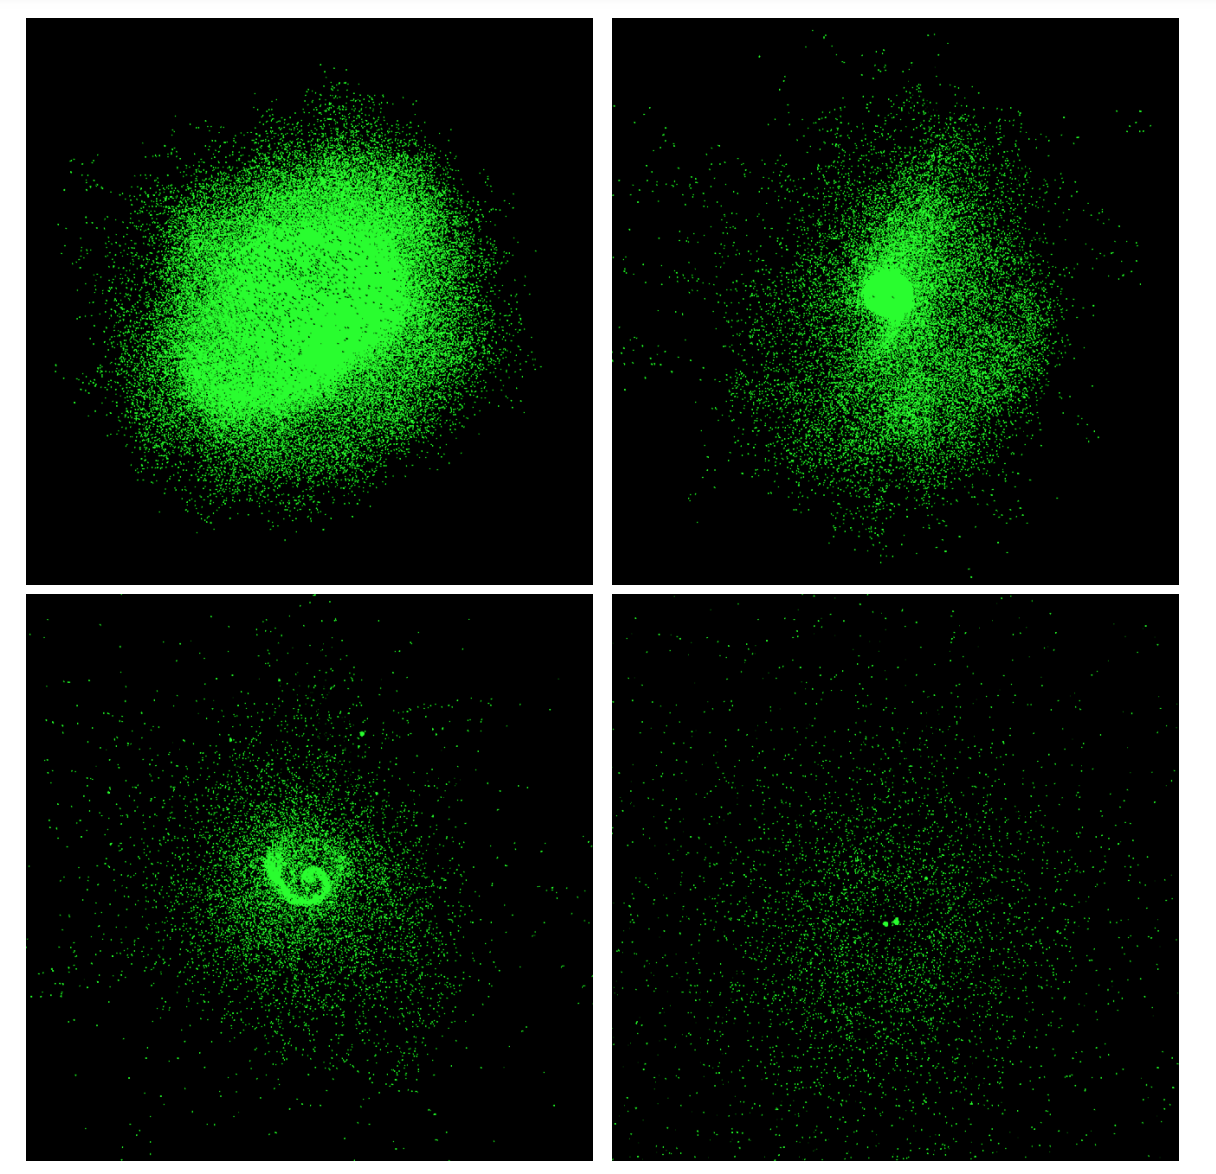
\includegraphics[width=\textwidth]{figures/intro/binaryPl.png}
    \caption{Simulation snapshots of a gravitationally bound pebble cloud formed via the streaming instability. Over the course of about 50 years (top left to bottom right), the clump collapses to form a binary planetesimal. (Adapted from figure 14 of \cite{nesvorny21})\label{fig:plCollapse}}
\end{center}
\end{figure}
 
Unfortunately, the conditions in simple models of protoplanetary disks are not sufficient to trigger the streaming instability. High resolution numerical studies suggest that dust to gas ratios larger than 4 percent are required to trigger it \cite{carrera15, yang17}, while the early solar system was thought to have a dust to gas ratio closer to 1 percent \cite{hayashi81}. This suggests that planetesimals should not be expected to form everywhere in the disk, although the fact that planets and smaller bodies, which presumably originated from planetesimals, exists everywhere from $\sim$ 0.5 to $\sim$ 50 AU in the solar disk. \textbf{It should be noted, that indirect measurements of the dust to gas ratio in planet forming disks exhibit a surprisingly wide range of values, some of which come close to the value required by streaming instability experiments \cite{rich21, jermyn22}.} Future, higher resolution studies of the streaming instability may \textbf{also} alleviate this discrepancy.

% Todo Eric: VSI or RDI (urpin, hopkins/squires)

Another solution to the problem of triggering the streaming instability may come from relaxing the assumption that the terrestrial planet forming regions of protoplanetary disks are smoothly varying. Pressure bumps in the gas disk, formed by mechanisms such as ionization fronts, condensation fronts, perturbations from other planets or self-induced dust traps \cite{gonzalez17} can all act to halt the inward drift of small solids and concentrate them into rings with conditions amenable to triggering the streaming instability \textbf{or} even gravitational fragmentation \textbf{\cite{chatterjee14, izidoro21, morbidelli21, batygin23a}}

\section{Observational Constraints}\label{sec:obsConstraints}

For $\mu$m to mm sized grains, scattered light from the central star, along with thermal emission allows us to directly trace this early phase of growth. For Earth-sized planets and larger, alterations to the light emitted by the host star allow us to observe the final outcome of the planet formation process. Populations of objects in between these sizes, however, do not have enough surface area to scatter light or emit appreciable amounts of thermal radiation, while being too small to perturb the light from the central star. With the exception of the remaining small bodies in the solar system, many of which are believed to be residual planetesimals, the gravitationally-dominated stage of the terrestrial planet formation process is essentially invisible.

In the solar system, the orbital configurations of the planets themselves contain clues that the small body population was once much more numerous. A model in which the orbits of Saturn and Jupiter gradually evolve due to repeated scattering events with smaller bodies and subsequently go unstable works well to explain the present day configuration of the Jupiter trojans, Kuiper belt objects and irregular satellites (cite Nice model). This suggests that the solar system was once filled with planetesimals. In addition, N-body simulations have shown that a collection 100 km sized objects placed throughout the outer solar system can induce the inward migration of Neptune's orbit while capturing the proper amount of small bodies into mean-motion resonance \cite{murrayclay06}.

For planet-forming disks around other stars, the primary way to infer the presence of planetesimals and planetary embryos is through dust emission. Although some of this dust is likely primordial, a large fraction of it is expected to be generated by collisions between the gravitationally bound planetary building blocks. Although the initial stages of planetesimal growth are not expected to create much dust, the eventual protoplanets that form act to stir up the remaining planetesimals, increasing collision velocities and producing destructive collisions \cite{kenyon04}. In 2020, the thermal emission of a transient dust cloud resulting from a planetesimal-planetesimal collision was observed for the first time \cite{gaspar20}.

\begin{figure}
\begin{center}
    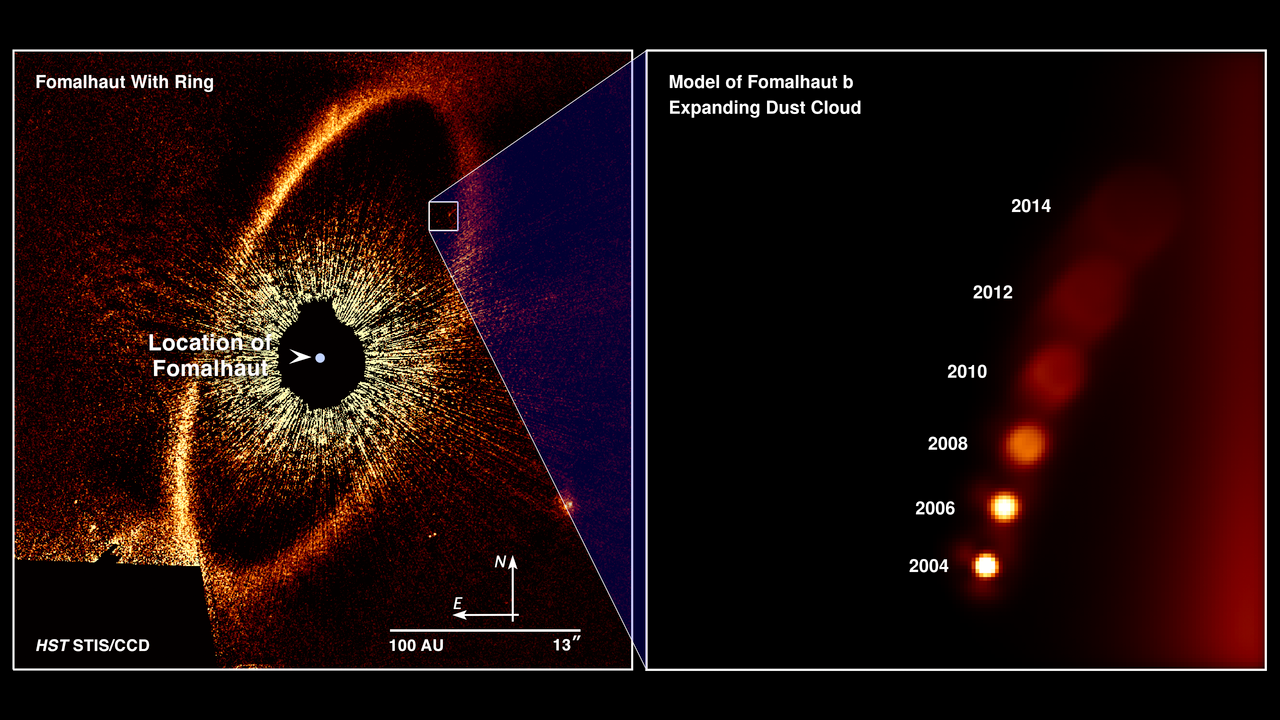
\includegraphics[width=\textwidth]{figures/intro/fomalhutb.png}
    \caption{A composite of archival images from the Hubble Space Telescope showing dust in scattered light surrounding the Fomalhut system. On the right, a closeup view of an expanding dust cloud, produced by a planetesimal collision is shown expanding over the course of 10 years. Image credit: NASA/ESA\label{fig:fomalhutb}}
\end{center}
\end{figure}

Often, the collisionally generated dust emission is used to infer the presence of an unseen planet. The intricate structure of bright rings and gaps seen in the planet-forming disk HL Tau \cite{alma15} have been argued to be indicative of three embedded giant planets \cite{boley17}. \cite{dobinson13, dobinson16} showed that the presence of a giant planet produces distinct morphological features in the collisionally generated dust emission, the properties of which can be used to constrain the orbital properties of the planet itself.

Despite \textbf{powerful} resolving capabilities ($\sim$ 1 AU resolution for the closest protoplanetary disks), sub-mm facilities like ALMA are not able to probe the terrestrial planet forming region of most disks. In fact, the inner 10 or so AU of most protoplanetary disks are optically thick at mm and shorter wavelengths \cite{beckwith90} and the conditions at the midplane where gravitationally bound solids are expected to form are completely hidden. Future radio observatories, such as the NG-VLA should be able to achieve sub-au resolution in the inner region of these disks \cite{ricci20}. In the meantime, constraints on planetesimal formation and terrestrial planet growth can only be attained by inward extrapolation of the solid distributions in the outer edges of observed protoplanetary disks, or by working backwards and reconstructing the conditions of the early solar system. Until better observational constraints can be obtained, smoothly varying power law models for the gas and solid distribution of the terrestrial planet formation regions remain a viable starting point.

% Todo: Erics comment about power laws overly simplistic

\section{Modeling Planetesimal Growth}

\subsection{Collision Rates and Runwaway Growth}

The problem of determining the outcome of planetesimal growth involves simultaneously evolving the mass distribution (as bodies collide and grow) and velocity distribution (as bodies gravitationally scatter) of the system. These models typically start with a collection of equal-mass planetesimals on nearly-circular, low inclination orbits about a much more massive central body. Predicting the evolution of the system requires a numerical approach, but some insights into the expected behavior can be obtained analytically. For an equal mass population of planetesimals with mass $m_{pl}$ and radius $r_{pl}$, the rate of change of the mass can be written as

\begin{equation}\label{eq:massgrow}
	\frac{dM}{dt} = \rho_{pl} v_{enc} \sigma = k \Sigma_{pl} \Omega \sigma,
\end{equation}

\noindent where $\rho_{pl}$ \textbf{and $\Sigma_{pl}} is the mass \textbf{and surface density} density of planetesimals at the midplane of the disk, $v_{enc}$ is the typical encounter velocity between bodies, $\Omega$ is the Keplerian orbital frequency and $k$ is a numerical pre-factor which captures the geometric effects of encounters in a disk. The effective collision cross section $\sigma$ is set by the geometric value and is enhanced by gravitational focusing, which bends the trajectories of planetesimals that undergo a close encounter.

\begin{equation}\label{eq:gf}
	\sigma = \pi r_{pl}^2 \left( 1 + \frac{v_{esc}^2}{v_{enc}^2} \right),
\end{equation}

\noindent where $v_{esc}$ is the mutual escape velocity of two planetesimals that are in contact at their surfaces

In the case where the planetesimal disk is dynamically cold ($v_{esc} \gg v_{enc}$), equation \ref{eq:massgrow} scales with mass as $dM/dt \propto M^{4/3}$. This implies that the growth rate accelerates with time and leads to a situation known as runaway growth \cite{wetherill89, kokubo96}.

\subsection{Two-body Relaxation}

At the same time, the encounter velocities in the disk evolve due to two-body relaxation. This is effectively due to gravitational encounters converting energy from the differential rotation of the disk into random motion. For an equal mass population of bodies, the timescale for relaxation can be written as 

\begin{equation}\label{eq:relax}
	t_{relax} = \frac{v_{enc}^2}{d v_{enc}^2 / dt} = \frac{v_{enc}^3}{\rho_{pl}^2 \pi G^{2} m_{pl}^4 ln \Lambda}
\end{equation}

\noindent where $G$ is the gravitational constant and $ln \Lambda$ is the Coulomb logarithm, which captures the effects of long-distance encounters and is typically taken to be $\simeq$ 10 for a planetesimal disk.

As the planetesimal system evolves, the assumption of equal-mass bodies is quickly violated. In this situation, a numerical approach is required. This was first done by \cite{greenberg78} and involves dividing growing planetesimals into bins of mass and distance from the central star and evolving them using a statistical approach. This method, which provided the first confirmation that runaway growth indeed persists beyond the initial equal-mass phase \cite{wetherill89}, suffers from a few severe limitations. First, dynamical effects such as energy exchange between bodies of different masses and encounters between slow-moving bodies which are strongly mediated by the gravitational field of the central object, must be explicitly built in to the model. Second, runaway growth naturally produces a power law tail of bodies. In this situation, the highest mass bins eventually end up with only a few bodies which dominate the dynamical evolution of the system and a statistical approach begins to break down.

\subsection{N-body Simulations of Planetesimal Accretion} \label{sec:nbodyPl}

The straightforward, albeit computationally expensive way to circumvent these problems is to instead evolve the equations of motion for the growing planetesimals individually. To do so explicitly requires pairwise force evaluations and collision checks between all bodies at every timestep. Given that these calculations naively require $O(n^2)$ evaluations per timestep, this can quickly become prohibitively expensive, especially considering that terrestrial planet formation timescales are on the order of Myrs, while dynamical timescales between planetesimals can be on the order of days. It took decades after the idea of runaway growth was first proposed before its effects and eventual end were directly simulated using an N-body code \cite{kokubo96, kokubo98}. Even then, the simulations were limited to a narrow annulus, where it was assumed that the growth modes scaled in a self-similar way throughout a full planetesimal disk.

The introduction of tree-based N-body codes such as {\sc pkdgrav} \cite{richardson00, stadel01, wadsley04} finally allowed for much larger particle counts to be used, in which planetesimals were much closer to the sizes predicted by formation models. By dividing physical space into subdomains, force calculations and neighbor lookups for collision detection can be done in $O (n log n)$ time using an algorithm similar to a Barnes-Hut tree \cite{barnes86}. 

The simulation code used to model planetesimal accretion in this thesis is called {\sc ChaNGa}, which is a descendent of {\sc pkdgrav}. {\sc ChaNGa} is actively being developed by the N-body shop at the University of Washington and is designed to \textbf{enable} force calculations and neighbor finding for huge collections of particles by efficiently distributing the work across machines running in parallel on a supercomputing cluster \cite{jetley08, menon15}. This is done by splitting groups of particles into objects called TreePieces, which are then assigned to different compute domains and are designed so that calculations on a given TreePiece can be done semi-independently. Much of the power of {\sc ChaNGa} comes from the fact that load balancing and communication between cores is handled in a very dynamic and efficient way. For cosmological simulations, {\sc ChaNGa} can easily handle upwards of billions of particles, although the much larger range of timescales that must be handled in a planetesimal accretion simulation restricts this to a few million.

% TODO: Erics question about particles in neighboring tree pieces

{\sc ChaNGa} is written in the {\sc CHARM++} programming language and has been shown to perform well when using up to half a million processors \cite{menon15} simultaneously. Gravitational forces are calculated using a modified Barnes-Hut tree algorithm with hexadecapole order expansions of the moments. For all of the planetesimal accretion simulations described in this paper, a node opening criterion of $\Theta_{BH}$ = 0.7 was used. In chapter \ref{ch:plSS}, I test the effects of varying $\Theta_{BH}$ on a planetesimal disk and show that the tree approximation does not meaningfully affect the influence of two-body encounters. The equations of motion are integrated using a kick-drift-kick leapfrog scheme. For more information about the implementation of {\sc ChaNGa} see \cite{jetley08}.

%\cite{richardson00} was able to resolve mean motion resonances in a terrestrial disc using a similar tree code with the same node opening criterion, so we expect that our model should properly handle resonance effects as well. (Move to ch2?)

In order to use {\sc ChaNGa} to study planetesimal coagulation, I implemented a hard-body collision model that treats particles as solid objects with a fixed radius, rather than as smooth tracers of a fluid with a characteristic softening length. The framework for the collision detection module uses the existing algorithm for neighbor finding during smooth particle hydrodynamics (SPH) calculations. As with the gravity calculations, particles are sorted into a tree structure which allows the collision search to be conducted in $\mathcal{O}(N\log{}N)$ time. The collision detection module in {\sc ChaNGa} based off of the solid body collision implementation in {\sc pkdgrav}, which is described in \cite{richardson94} and \cite{richardson00}, which we summarize below:

Collisions are predicted at the beginning of each drift step by extrapolating the positions of the particles forward using the velocities calculated during the first kick. For each particle, the closest 64 neighbors are considered in the collision search. After extrapolating the positions forward and checking for overlap with any neighbors, the earliest collision time $t_{coll}$ is stored for each particle.

After the prediction phase, particles with $t_{coll}$ less than the time step size $\Delta T$ must have their collisions resolved. For simplicity, all collisions in our simulations result in perfect accretion. A merger between two particles of mass $m_{1}$ and $m_{2}$ results in a single particle of mass $M = m_{1} + m_{2}$, with the radius set to conserve density. The position and velocity of the resulting particle is set to the centre of mass position and velocity of the colliders at the moment of contact. The resulting merged particle is then drifted to the end of the step. If multiple collisions are predicted during a time step, the earliest collision is resolved first. Because resolving a collision can result in another imminent collision, collisions must be resolved one by one, with a new prediction check being run each time.

\subsection{N-body Simulations of Final Planet Assembly}

Although tree-based N-body codes work well for modeling planetesimal accretion, the later stages of terrestrial planet formation, in which protoplanets collide to form planets, requires integrating through prohibitively large number of dynamical times (on order $10^{10}$ timesteps). During this phase, collisions and close gravitational encounters are rather infrequent. During timesteps where there are no close encounters, a mixed variable symplectic \textbf{(MVS)} integration scheme can be used \cite{wisdom91}. This involves splitting the Hamiltonian of \textbf{a} system into a Keplerian and perturbing part. These two parts can be solved independently, the former of which is done analytically and can be done orders of magnitude more quickly than solving the equations of motion using a direct $O(n^{2})$ or a tree-based approach. In cases where a close encounter occurs, the perturbing term in the Hamiltonian becomes large and the motion of the interacting particles is solved directly. This hybrid integration scheme was first implemented in the code {\sc Mercury} \cite{chambers99} and allowed for the first time planet formation simulations using hundred to thousands of particles.

 Restricting planet formation simulations to begin with no more than a few thousand particles, is still quite limiting. Due to this restriction, these types of simulations are often built with rather unrealistic initial conditions, in which planetary embryos are already fully formed in the disk and residual planetesimals are either represented by super-particles, or their gravitational influence is ignored. Recent advances in GPU hardware, however, have allowed more recent N-body codes to push beyond these limitations. In particular, the N-body code {\sc genga} \cite{grimm14, grimm22} has been developed to specifically take advantage of GPU hardware for running a hybrid MVS integrator up to 30 times faster than {\sc Mercury}. Recent versions of genga are able to efficiently handle prolonged close encounters between large groups of particles and the code has been successfully used to model the coalescence of tens of thousands of fully self-interacting particles into a system of terrestrial planets \cite{woo21}.

\section{Thesis Goals and Outline}

In this thesis, I present my work using high resolution N-body simulations to understand the dynamics and outcome of the planetesimal accretion process. I will begin by connecting this process to the present-day small body populations in the inner solar system, particularly the asteroid belt. Then, I examine the role that planetesimal collisions play in the generation of debris disks. Lastly, I follow the growth of a planetesimal disk into a fully-formed system of short-period planets. From here, I make connections with the compact, multiplanet systems observed by Kepler and TESS to understand how viable a migration-free terrestrial planet formation model can be in this context.

\subsection{Chapter 2 Summary}

In chapter 2, I revisit the problem of planetesimal accretion in the inner solar system starting with near-realistic sized bodies. I show that the post-runaway growth phase is resolution dependent and that finely-spaced mean-motion resonances with the largest bodies are only populated if the planetesimal population is sufficiently fine-grained. In the case where this condition is met, the mass distribution of the residual planetesimal population follows a broken, rather than a single power law. This is strongly reminiscent of the mass distribution of the present day asteroid belt and Kuiper belt and I demonstrate that subsequent collisional destruction is not the only pathway to produce such a break.

\subsection{Chapter 3 Summary}

In chapter 3, I follow the orbital evolution of a planetesimal belt in the vicinity of a giant planet and use the recorded collision rates to construct a dust emission map. Near the locations of mean-motion resonances, distinct overdensities or underdensities in the dust can form. The mapping between particular resonances and the presence of a gap or bright ring in the dust emission is shown to depend on the mass and eccentricity of the giant planet. I show that from the dust emission alone, it is possible to constrain the orbital properties of the giant planet.

\subsection{Chapter 4 Summary}

In chapter 4, I simulate the planetesimal accretion process at short (1 to 100 day) orbital periods and show that the gravitational interactions that facilitate energy equipartition and eventually shut off the runaway growth phase become ineffective close to the star. I show that a disk of rocky planetesimals should be expected to undergo two distinct accretion modes, with the boundary lying around 5 to 10 days in orbital period. This result has implications for the expected configuration of planetesimals and embryos at the beginning of the giant impact phase and suggests that the initial conditions used for short-period planet formation simulations are often overly simplistic. In the following chapter, I use these simulation results to explore the effect that this accretion boundary in the disk has on the final assembly of the planets.

\subsection{Chapter 5 Summary}

In chapter 5, I use the final simulation snapshots from chapter 4 to grow the remaining planetesimals and protoplanets into a fully-formed system of terrestrial planets under a migration-free model. These are the first-ever simulations in which the planet formation process is followed from the smallest gravitationally bound bodies (planetesimals) to full-sized planets. Having directly resolved every collision, I map the building blocks of the planets back to their original locations in the disk to assess the extent of radial mixing in the disk. Due to the computational expense of the planetesimal accretion simulations, I train a neural network on the results from the previous chapter and use it to produce a much larger set of intermediate-phase initial conditions which are then run and used to capture the effects of stochasticity and chaos during the giant impact phase.
